% Template for PLoS
% Version 1.0 January 2009
%
% To compile to pdf, run:
% latex plos.template
% bibtex plos.template
% latex plos.template
% latex plos.template
% dvipdf plos.template

\documentclass[12pt]{article}

% amsmath package, useful for mathematical formulas
\usepackage{amsmath}
% amssymb package, useful for mathematical symbols
\usepackage{amssymb}

% graphicx package, useful for including eps and pdf graphics
% include graphics with the command \includegraphics
\usepackage{graphicx}
\usepackage{epstopdf}
\usepackage{color}

% cite package, to clean up citations in the main text. Do not remove.
\usepackage{cite}

% Use doublespacing - comment out for single spacing
\linespread{1.5}

% Text layout
\topmargin 0.0cm
\oddsidemargin 0.5cm
\evensidemargin 0.5cm
\textwidth 16cm 
\textheight 21cm

% Use the PLoS provided bibtex style
\bibliographystyle{plos2009}

% Remove brackets from numbering in List of References
\makeatletter
\renewcommand{\@biblabel}[1]{\quad#1.}
\makeatother


% Leave date blank
\date{}

\pagestyle{myheadings}
%% ** EDIT HERE **


%% ** EDIT HERE **
%% PLEASE INCLUDE ALL MACROS BELOW

%% END MACROS SECTION

\begin{document}

% Title must be 150 characters or less
\begin{flushleft}
{\Large
\textbf{Computational Identification and Annotation of Key-reactions in Metabolic Pathways of E. coli that Discriminate Different Growth Conditions.}
}
\bigskip
\noindent
% Insert Author names, affiliations and corresponding author email.
\\
Viswanadham Sridhara$^{1}$,
Austin G. Meyer$^{1,2,5}$,
Piyush Rai$^{3}$,
Jeffrey E. Barrick$^{1,2}$,
Pradeep Ravikumar$^{3}$,
Daniel Segre$^{4}$, 
Claus O. Wilke$^{1,5,\ast}$
\\
\bigskip
\bf{1} Center for Computational Biology and Bioinformatics, The University of Texas at Austin, Austin, TX, USA
\\
%\\[3\baselineskip]
\bf{2} Department of Chemistry and Biochemistry, The University of Texas at Austin, Austin, TX, USA
\\
%\\[3ex]
\bf{3} Department of Computer Science, The University of Texas at Austin, Austin, TX, USA
\\
%\\[3ex]
\bf{4} Department of Biology, Boston University, Boston, MA, USA
\\
%\\[3ex]
\bf{5} Section of Integrative Biology, The University of Texas at Austin, Austin, TX, USA
\\
%\\[3ex]
\bigskip
$\ast$ E-mail: wilke@austin.utexas.edu
\end{flushleft}
%\\
% Please keep the abstract between 250 and 300 words
\newpage
\begin{abstract}
Currently, predicting bacterial growth conditions without prior knowledge of the medium is an unresolved problem. By contrast, computing bacterial metabolic output, given a set of starting conditions has become a comparatively routine task via flux balance analysis (FBA). To compute metabolic output, one specifies a set of starting conditions within the context of a complete bacterial metabolic model. Here, we selected 7 carbon and 7 nitrogen sources along with 4 more commonly used experimental media. We generated metabolic flux data using FBA in E. coli MG1655 for the 18 specified growth conditions. We then used a model selection algorithm to identify the key reactions that discriminate among the tested growth conditions. These models on average require assaying the fluxes through 9 reactions to accurately predict the correct carbon and nitrogen source used during growth. For each source metabolite, we mapped its predictive reactions onto the E. coli central carbon metabolism to highlight important metabolic regions. Our analysis provides several important physiological and statistical insights. First, by analyzing metabolic end products, we can consistently predict growth conditions. Second, despite its heterogeneity, the experimental media appears to be similarly predictable to the homogeneous media. Third, predictive reactions seem to frequently lie near the initial entry point into central metabolism for the metabolite being predicted. Finally, we found that separately predicting the carbon and nitrogen sources is better than making joint predictions. In addition, the fact that separate prediction performs better than a more sophisticated joint prediction scheme, generates several potentially interesting hypotheses regarding bacterial physiology.
\end{abstract}

% Please keep the Author Summary between 150 and 200 words
% Use first person. PLoS ONE authors please skip this step. 
% Author Summary not valid for PLoS ONE submissions.   

\section*{Author Summary}
%Predicting the biomass composition, co-factors yield using FBA techniques on computational metabolic models is gaining popularity in the last decade. Moreover, metabolic pathways provide us a framework to integrate diverse kinds of high-throughput data i.e., transcriptomics/proteomics/metabolomics data. Here, we generated metabolic fluxes for different growth conditions and then used machine learning techniques to predict the key-reactions that discriminate different growth conditions. Such automatic identification of key-reactions would in turn also help experimentalists to quantitatively measure the respective metabolites involved (mass-spec based metabolomics), proteins that catalyze the reactions (mass-spec based proteomics) or the genes that encode these enzymes (sequencing based RNA-seq experiments).

\section*{Introduction}
Flux balance analysis (FBA) is a computational technique that is routinely used for computational guidance in metabolic engineering \cite{Orthetal2010}. Traditionally, FBA involves training a whole-cell metabolic model with a specified starting media and optimizing the network to produce a specific output. The goal of such analyses is to identify bottlenecks to producing various metabolic products. 

%FBA requires a metabolic model, which generally is obtained from genome sequence and its annotations. The metabolic models of few species are well developed over the past decades, given the advances in genome sequencing \cite{Schellenbergeretal2010,Caspietal2012}. Determining enzyme kinetics for metabolic reactions is extremely difficult and hence constrained based methods like FBA that calculate steady-state flux vector have gained importance.

%The genome sequence, its annotation along with the massive amounts of biochemical data available from the literature are the key ingredients for metabolic reconstructions \cite{EdwardsPalsson2000, Karpetal1996, OuzounisKarp2000}. Among prokaryotes, E. coli metabolic model has been very well annotated  by several groups \cite{Karpetal1996,EdwardsPalsson2000}. Palsson's group has been extensively updating the E. coli metabolic model over the last 2 decades \cite{EdwardsPalsson2000,Reedetal2003,Feistetal2007,Orthetal2012}. Similarly Karp's group at SRI is updating their model for more than 2 decades and stored the content as EcoCyc pathway genome database \cite{Keseleretal2013}. 

%At the same time, the experimental data can be used to refine the constraints used in these flux balance analysis. Recently, gene expression profile data is used to refine the bounds of reaction fluxes in metabolic models, which in turn helped improve prediction of input carbon sources \cite{Brandesetal2012}. There is still lot of room for improvement, given the different kinds of possible constraints \cite{Priceetal2004}.

%There was a study that identified minimal set of reactions that are necessary for growth for a particular growth condition \cite{Burgardetal2001}. Likewise, there was another study published recently that identified minimal set of nutrients for growth conditions \cite{Ekeretal2013}. Another study by Ibarra et. al., \cite{Ibarraetal2002} looked at the growth of E. coli K-12 MG1655 strain on glycerol for 40 days (~700 generations) and they saw an increase in the growth rate with generations. These are some of the studies that indicate diverse applications of metabolic engineering that use FBA.

%The metabolic pathways, apart from providing a genotype-phenotype relationship, also provide a good resource to integrate diverse kinds of data, such as DNA sequence, mass-spectrometry data. For example, combining flux analysis data with phosphoproteomics data to deduce functionality of enzymes is described in this study \cite{Oliveiraetal2012}. An interesting study to understand the adaptation of yeast metabolism to the growth conditions is studied, using enzymes in metabolic model pathways to validate the quantitative proteomics data \cite{Costenobleetal2011}. Other than the above studies, this set of pathways when integrated with other diverse types of data, have many applications as discussed in these 2 reviews \cite{Hydukeetal2013,Oberhardtetal2009}.

%As shown by \cite{Almaasetal2004}, for a particular design (growth type/mutant etc) there are many reactions that have low reaction flux, but the ones with high-flux typically provide information on the growth condition or the mutant type. To our knowledge, there were no studies that identified growth sources from flux data. Here, we used machine learning techniques to predict these sources from patterns of simulated flux data.

%Machine learning algorithms use with computational biology has been growing. In biological data, generally the number of samples is far less than features. So, linear models cannot be used without reducing the number of covariates.  For example, differential expression of tens of thousands of genes in microarray studies or identifying the SNPs in GWAS studies is a routine task in biomedical research now-a-days. Even though the sequencing technologies are becoming cheaper day-by-day, the number of samples sequenced is still low, compared to the number of features. In such cases, model selection algorithm LASSO \cite{Tibshirani1996} seems to perform well. LASSO methods are used in the past for genomics studies \cite{Wuetal2009}. LASSO seems to perform well with other kinds of data, for example, classifying structural images of brain using MRI data \cite{Casanovaetal2011,Casanovaetal2012,Wangetal2012}.

%There are many R and MATLAB packages that can be used for LASSO. GLMNET  \cite{Friedmanetal2010} is one such package that can be used for methods based on convex penalties (lasso, ridge-regression, elastic net etc). This package also comes with algorithmic efficiency and speed \cite{Friedmanetal2010}. GLMNET is shown to work on large datasets and with many labels. Given the sparsity of the reaction flux data, we used GLMNET \cite{Friedmanetal2010} for classifying different growth conditions.

\section*{Results}
\subsection*{Predicting growth conditions from simulated flux in \emph{E. coli}}

We wanted to know to what extent bacterial physiology reflects specifics about the growth environment. In other words, if we have measured the physiological state of a bacterium, can we deduce under what conditions it was grown? Here, we addressed this question in a simulation framework, using flux-balance analysis (FBA) as our model for bacterial physiology. Our overall strategy was as follows: (i) simulate metabolic fluxes under a variety of different growth conditions (primarily distinct carbon and nitrogen sources); (ii) develop regression models that regress the growth conditions against the calculated metabolic fluxes; (iii) evaluate how accurately the regression model can predict growth conditions from fluxes.

One inherent challenge with our approach is that flux-balance models do not allow for promiscuous reactions. Each reaction in the model has a small and unique set of reactants and a similarly minimal set of products. A biochemically similar reaction on a different substrate is represented as a separate reaction in the model. Further, substrates are brought into the cell and transported among different compartments in the cell via \emph{transport reactions}, which simply take up a molecule of a specific metabolite in one compartment and release that same molecule in another compartment of the cell. Thus, any metabolic flux model contains a substantial number of transport reactions whose sole purpose it is to get specific metabolites into the cell. Clearly, predicting environmental growth conditions from fluxes through these transport reactions would be trivial, and it would not be a reflection of what information the internal metabolic state of the cell holds about the external environment. To address this issue, we discarded all transport fluxes in our regression analysis. In our model (iAF1260 metabolic model of the \emph{E. coli} K-12 MG1655 strain \cite{Schellenbergeretal2010}), this amounted to {\color{red}please insert number} among a total of 2382 distinct reactions.

Further, to make the task of predicting growth conditions from fluxes more difficult and more realistic, we introduced background contamination in all simulated environments. Each environment consisted of a set of primary metabolites (usually one carbon and one nitrogen source) plus a small quantitiy of randomly chosen other metabolites. We varied the number of contaminant metabolites to evaluate how sensitive the regression model was to the amount of background contamination. Contaminant sources were selected at random from a set of 174 carbon and 78 nitrogen sources used previously with the \emph{E. coli} model \cite{Feistetal2007}. A different set of random contaminants was chosen for each individual FBA calculation.

We first wanted to test how well prediction might perform in a best-case scenario. To this end, we selected seven carbon and seven nitrogen sources ({\color{red}Table X}) that generated substantially distinct flux patterns in the absence of contaminants. We assessed the similarity of flux patterns by $k$-means clustering of fluxes obtained for all 174 carbon and 78 nitrogen sources (data not shown). We then generated fluxes for environments with contaminants for all pairwise combinations of the seven carbon and seven nitrogen sources. We generated 100 replicates of each pairwise combination, for a total of 4900 total sets of flux values. {\color{red}We discarded solutions that we considered to be non-viable?} 

{\color{red}Copy-edit from here.}

Next, we generated a training set by randomly drawing from our simulated fluxes. We trained the models with a generalized linear model to predict starting conditions based on final fluxes. The remaining simulation data was used to calculate the misclassification rates. We used cross-validation in a generalized linear model to pick regression coefficients. 

\textbf{Should we report something about the regression method?}

We found that even at relatively high noise levels of 10\%, we are able to predict the growth media in greater than 80\% of cases. Figure~\ref{fig:misclassification_1} illustrates that as random background carbon and nitrogen sources are added, the misclassification rate increases relatively little. Moreover, assuming a training set of sufficient size, it appears additional data does little to affect the accuracy of model predictions. Despite our simulations being run as pairwise combinations of the available carbon and nitrogen sources, there appears to be no benefit to joint prediction. In fact, a model involving the separate prediction of the carbon and the nitrogen sources performed better in all cases tested here (Figure~\ref{fig:misclassification_1} and Figure~\ref{fig:misclassification_2}). Unsurprisingly, at the lowest noise tested, the difference between joint and independent predictions is at a minimum; by contrast, at 10\% noise the difference climbs to greater than 10\% of the total misclassification rate (Figure~\ref{fig:misclassification_2}). Despite the comparatively poor performance of joint prediction, with a 10\% noise level and joint a joint prediction algorithm, the misclassification rate tops out at 25\%. By contrast, by random chance one would only expect to choose the correct growth condition in approximately 2\% of cases or alternatively misclassify growth conditions 98\% of the time. In addition, within the range of training set size we tested, the relative value of more data for separate prediction was substantially lower than for joint prediction.

In order to generalize our simulations to more experimentally relevant test conditions, we performed similar analyses for several media that are more commonly used in experimental microbiology. Specifically, we tested autoinducer bioassay (AB) minimal media, proprietary media from the company ATCC, Davis Mingioli (DM) media and Bochneder defined minimal media. Due to the relatively small number of available starting conditions in the training set, we were able to classify our experimentally relevant media choices very accurately. Our misclassification rate was less than 1\% for noise levels up to 20\%. \textbf{(Viswanadham, what does this sentence mean???) There was only one feature predicted for each of 3 reactions, except for AB minimal media, for which only $\beta_0$ is non-zero and the rest of regression coefficients are 0}. 

\textbf{(We should add some more... perhaps the commented text below, but we'll need to clean it up.)}

%Not sure what to do with this paragraph.  Is the analysis finished and available?
%Since individual prediction is shown to perform better than joint prediction, we did large-scale prediction of the comprehensive list of 174 carbon and 78 nitrogen sources. We used the similar methodology as we used earlier i.e., we generated simulated fluxes for all pair-wise combinations of carbon/nitrogen sources (174*78) for 2 replicates. We used 1 replicate for training the model and then we used the 2nd replicate for testing. The misclassification rate for carbon sources is X\%, while the misclassification rate for nitrogen sources is Y\%.  

\subsection*{Application to experimental design}

To gain some mechanistic insight into predictive reactions, we mapped them onto the E. coli central metabolism model. The predictive reactions were overlayed on E. coli MG1655 central metabolism. Manual validation of these reactions indicate that most reactions seem specific to some unique growth source. For example, using acetate as the carbon source unsurprisingly isolates TCA cycle entry as a predictive reaction. Similarly, sorbitol is the singly reduced alcohol of D-glucose and fructose enters glycolysis just three steps away from un-phosphorylated D-glucose; thus, each possesses a predictive reaction in the relative vicinity of the glycolytic pathway (Figure~\ref{fig:carbon_network}). Mapping nitrogen sources to central metabolism reveals a similar trend. For example, L-alanine as a growth source has predictive reactions near its site of entry into the three and four carbon metabolism of the TCA cycle (Figure~\ref{fig:nitrogen_network}). Each of the metabolic maps (Figure~\ref{fig:carbon_network} and Figure~\ref{fig:nitrogen_network}) is meant to highlight generally important areas in the E. coli central metabolism.

Despite the accuracy of our scheme, a model with a large number of predictive reactions would quickly become intractable in experimental applications; after all, each predictive reaction means an additional unique biochemical assay. Our model required an average of 9 reactions for accurate prediction. Considering our network included a total of 1443 reactions after transport reaction removal, 9 is an impressively minimal requirement for media prediction. To understand the effect of reducing model parameters below the optimal number, we employed a different strategy from that used above. There were 126 reactions that were assigned a non-zero coefficient in our trained model. For each of those 126 reactions, we eliminated one at a time, trained a new model, and calculated the test accuracy. With the exception of 3 reactions, we found that the misclassification rate remained unchanged for each of the other 123 reactions. Thus, the feature selected average of 9 predictive reactions very likely does not represent a unique solution. More importantly, for experimental purposes, the number of assayed reactions could very likely be further reduced without sacrificing much predictive power.

%this paragraph is out of place and I'm not sure what it tells us.
%As a further test, we obtained simulated flux measurements using maltose as carbon source and the 7 nitrogen sources used earlier. Individual prediction seems to classify maltose as glucose more than 85\% of the times. The nitrogen sources were predicted correctly more than 95\% of the times. However, when we tried to predict using the joint model, the nitrogen sources were mispredicted most of the times. The carbon source 'maltose' was predicted as D-sorbitol most of the times. On the other hand, most of the nitrogen sources were predicted as putrescine. 

\section*{Discussion}

We have developed a method for making predictions regarding growth media from known metabolic flux data. We generated fluxes by simulating the complete E. coli metabolic network for 7 carbon, 7 nitrogen, and 4 experimental mixed media types. Then, we divided the data and employed machine learning with a generalized linear framework to train a model to predict growth conditions. We found that even at high noise levels, we could make reliable predictions regarding growth media for all of the sources we tested. Also, extending our prediction algorithm to more experimentally relevant growth media, our scheme gave comparable accuracy. Of note, our data indicates separately predicting carbon and nitrogen sources always performed better than joint prediction as paired input. Although this result is to some extent influenced by the volume of training data, it very likely says something important about rate-limiting reactions in the E. coli metabolic network. In addition, our results indicate that for most input metabolites at least one predictive reaction commonly occurs near its entry point to central metabolism. Finally, we found that the number of reaction fluxes required to make accurate predictions is relatively small and can probably be reduced further with few trade-offs. Thus, we have shown that predicting growth conditions from metabolic flux data is an experimentally tractable problem.

We have shown that given simulated metabolic flux data, growth conditions can be accurately predicted via machine learning. Although the fractional noise can have a dramatic affect on model accuracy, the misclassification rate remains acceptably low even with 10\% or 20\% noise. The addition of noise revealed one interesting and unexpected physiological hypothesis about E. coli metabolism. Namely, as noise increases from 1\% to 20\%, our model increasingly predicts acetate as the default carbon source and ammonia as the default nitrogen source.  Due to its centrality in terms of energy production, for any input growth source the reactions that lead to the TCA cycle should have some reasonable amount of reaction flux. In order words, acetate and ammonia as default nutrient sources may not be so surprising when one considers acetate's central role in the TCA cycle--it is essentially the center of bacterial metabolism. Further, ammonia is one of the few, if not the only, source of nitrogen without any associated carbon atoms; as a result, it is unique among the input nutrient sources we tested. \textbf{(Maybe another sentence to connect thoughts)}. To be sure that the observed default carbon source misclassification was not an artifact of nutrient limitation (carbon versus nitrogen), we changed the uptake rates of carbon and nitrogen sources so that there was no limiting factor and re-analyzed by training a new model. Reversing nutrient limitations appears to have no effect on the default behavior of our trained model.

It was surprising to us that given the same number of observations in the training set, separate prediction of starting materials always performed better than joint prediction. There are two likely explanations for this result. First, making joint predictions requires discriminating between 49 different pairwise combinations. By contrast making individual predictions only requires discriminating 7 different conditions in two different sets. Thus, one possible explanation for the lack of predictive power is that we simply did not have the appropriate level of training data. Indeed adjusting the amount of training data appears to have a dramatic effect on joint prediction in particular (Figure~\ref{fig:misclassification_1}). On the other hand, such an issue represents an important experimental concern. Often the size of the training set, being experimentally determined, is just as limiting as the size of the testing set. As a result, our analysis indicates employing a separate prediction strategy will generally be more useful for experimental application. Second, although the mechanism is not completely clear to us, separate prediction may gain additional power due to the physiology of the organism. For example, if the initial, metabolite unique, steps of metabolic entry are often predictive (as they appear to be), running independent predictions would be expected to perform better per amount of data; in essence such a prediction strategy makes the assumption that pathways for the various metabolites are largely disconnected. By contrast, if one were using a single metabolite as a combined carbon and nitrogen source, we may expect an independent prediction strategy to perform relatively poorly as the independence assumption is not satisfied.

In this study, we used a relatively common machine learning technique called Lasso to prevent over fitting during feature selection in the regression model. To our knowledge, Lasso methods have not previously been applied to analyze metabolic pathways. By contrast, there are studies applying Lasso to other biochemical networks such as gene regulatory networks \cite{Menendezetal2010} and \textbf{(Viswanadham, there needs to be something else to make the sentence structure flow well)}. We would like to point out that beyond Lasso there are a number of other commonly used regularization techniques. For example, graphical Lasso \cite{Friedmanetal2008} and Ising Markov Random Field models \cite{Ravikumaretal2010} can \textbf{(...do something that I'm not really sure about)}. \textbf{(Viswanadham, I'm not sure if this is accurate... if not, we should say why we chose lasso.)} We chose Lasso because it provides a relatively simple and particularly robust framework for feature reduction. Thus, considering the large size of our simulation model, we were able to achieve a remarkbly small number of source-predicting reactions.

Finally, we have shown that there is no obvious experimental restriction for applying FBA and machine learning to predict initial growth media from final metabolic flux data. Nine reaction fluxes on average provided the optimal solution to our regression model; however it is evidently not a unique solution. There are very likely other possible alternative solutions that may garner similar predictive power. By individually eliminating reactions and retraining the model, it appears the minimum number of critically important reactions is three for E. coli MG1655.  With such a small number of necessary reactions for gaining predictive power in reverse flux balance analysis, it should be possible to immediately apply this technique to experimental prediction. 

%agm haven't gone through methods yet.
\section*{Materials and Methods}
We used MATLAB and R for this study. For flux balance analysis, we used COBRA toolbox \cite{Schellenbergeretal2011} with MATLAB and for multinomial regression, we used GLMNET package \cite{Friedmanetal2010} with R. The methods are described in detail below.

\subsection*{Flux Balance Analysis:} 
In FBA, the steady-state solution for reaction fluxes is calculated. S(m,n) is the stoichiometric matrix for "m" metabolites and "n" reactions and is represented as S hereafter. The other variables used are v and x, where v is a vector of reaction fluxes for all the reactions involved and x is the concentration of the metabolites. In steady-state, the rate of change of metabolite concentrations is 0. So, we can formulate the above problem with the set of equations, as described below:

\begin{align}
dx/dt = Sv_{i}, \\
Sv_{i}=0.
\end{align}

The constraints that are typically used are: 
\begin{align}
\alpha_{i}<v_{i}<\beta_{i}
\end{align}
where $\alpha$ and $\beta$ are lower and upper bounds of the reaction fluxes.

Hence, we solve this set of linear equations with interested constraints by linear programming.
\begin{align}
{max.} c^Tv, s. t Sv_{i}=0.
\end{align}
where $c^Tv$ represents the biomass composition reaction.

Generally in these metabolic networks, the number of reactions are more than number of metabolites resulting in multiple solutions.  However in metabolic engineering applications, we are interested in optimizaing a certain function, for example here, we are interested in maximizing biomass composition which would result in a particular solution. 

Our motivation to introduce noise is 2-fold. First, we would like to find alternate optimal solutions using FBA methods so that the final prediction results still hold for varying noise levels. The second reason is to simulate replicates for a particular growth condition to train the mathematical models. Flux variability analysis can also be used for finding alternate optimal solutions, but apart from generating alternate optimal solutions and generating replicates, we can also introduce noise and find its effect in key-reaction prediction using the method described above.

\subsection*{E. coli model:} 
From the BiGG database, we downloaded the iAF1260 model, as it has shown to be used rigorously in various studies involving metabolic engineering and seems to agree well with the experimental data. Generally these models are stored in SBML format, which is becoming a common format for systems biology related models i.e., signaling pathways, gene regulatory networks, metabolic pathways etc \cite{Huckaetal2003}. In the current iAF1260 model, there are 2382 reactions, 1668 metabolites. The biomass composition reaction is also included in the model. Except for the input growth sources (Carbon and nitrogen sources used in this study) used, we did not change any defaults that are used in this model. The upper bounds on 2377 reactions is set to 1000 mmol/gDWhr, i.e., there is no limit on the production of metabolites involved in these reactions. But for 5 reactions, i.e., ATPM, CAT, FHL, SPODM, SPODMpp, the upper bound was set to 50 mmol/gDWhr. On the other hand the lower bound for almost 1800 reactions is set to 0 mmol/gDWhr, which means these reactions cannot uptake any metabolites from the media. For ATPM reaction, the lower bound is set to be the same as upper bound at 8.39 mmol/gDWhr. For the rest, the lower bounds were set to -1000 mmol/gDWhr, except for glucose and oxygen. We did not change the oxygen uptake rate (-18.5mmol/gDWhr), but we set the lower bounds of glucose and ammonia to zero. If we used glucose/ammonia as growth sources, we then set the lower bounds of these sources accordingly.

\subsection*{Growth conditions:} 
We picked the growth conditions manually from \cite{Feistetal2007} that seemed more common in experiments. In our study, we used pairwise combinations of 7 carbon sources, and 7 nitrogen sources. 7 carbon sources when used alone did not result in any growth. On the other hand, the nitrogen sources except ammonia contributed to E. coli biomass composition that is non-zero. These carbon and nitrogen sources are listed in Table I. Depending on the input growth, we set the lower bound of that particular exchange reaction to -20 mmol/gDWhr. This lower bound of -20 mmol/gDWhr is previously used as reasonable uptake amount in many studies \cite{Feistetal2007}. For 49 pair-wise combinations of the sources, we generated 100 replicates of data. Apart from these growth conditions, we also used 4 growth media, generally used in E. coli K-12 MG1655 experiments as cited in EcoCyc database [Cite URL of EcoCyc].

We changed the uptake rate of nitrogen source to -1000 mmol/gDW/hr, keeping the carbon source at -20mmol/gDW/hr to make sure carbon sources don't lack nitrogen source. We also repeated the analysis keeping the carbon source uptake at -1000 mmol/gDW/hr and nitrogen source uptake at -20mmol/g/DW/hr. 

\subsection*{Background noise levels:} 
To generate replicates and may be alternate optimal solutions using these conditions, we incorporated different background noise levels. For this, we used a subset of the 174 carbon and 78 nitrogen sources, previously used in Feist et. al \cite{Feistetal2007}.  We used different background noise levels, ranging from 1\% to 20\%. For example, if we want to set 5\% noise level, we randomly picked 5 Carbon and 5 nitrogen sources and set their lower bounds to -0.2 mmol/gDW. Please note that we generated the flux data for a pairwise combination of 1 carbon and 1 nitrogen source along with the background noise as described here. 
%[Since we are using different noise sources, we used a minimum threshold for biomass composition (0.558)].

For each noise level, we used half of the dataset as test set. We used subsets of the remaining half as training (i.e, 240,480,2400 observations). On the training sets we did 3-fold cross validation. We used cross-validation in GLMNET package for model selection. Model selection means picking the regression coefficients at the lambda value that had the lowest misclassification rate with 3-fold cross-validation. We then used this model to calculate the misclassification rate on the test set. We repeated this step to calculate the misclassification rates at different noise levels (1\%,5\%,10\%) and different training data sizes (240,480,2400 observations).

\subsection*{Regression based on regularization:} 
We used GLMNET package with R. We used 3 fold cross-validation. From the flux balance analysis, the observations we generated for different noise levels were divided into 2- halves, one for training and the other for test set. We did training and 3-fold cross validation to pick the lambda that has the lowest misclassification rate using the GLMNET. We did this for both joint prediction as well as the separate prediction and then making a joint call.

\bigskip
\noindent
1. Separately:
\noindent

i) Take data set
\noindent

ii) Train model to predict C sources
\noindent

iii) Train model to predict N sources
\noindent

iv) Predict C and N separately and calculate joint prediction accuracy.

\bigskip
\noindent
2. Jointly
\noindent

i) Take data set
\noindent

ii) Train model to predict C and N jointly
\noindent

iii) Predict C and N jointly and calculate prediction accuracy.

\bigskip
\noindent
Since the cross-validation accuracy cannot be used to compare the GLMNET results for separately predicting to that of joint prediction, we used the test set to determine the prediction accuracy.

\bigskip
\noindent
Below are the equations used in multinomial regression setting. If Y is a categorical response variable with "m" levels (m>2), and x is a predictor, this will result in
\begin{align}
log P_r(Y=l/x)/P_r(Y=m/x) = \beta_0l+x^T\beta_l, l=1,2,...,m-1.
\end{align}

From this, we can model
\begin{align}
P_r(Y=l/x) = e^( \beta_0l+x^T\beta_l)/\sum\limits_{k=1}^m e^( \beta_0l+x^T\beta_l).
\end{align}

The above model can be fit by maximizing the penalized log-likelihood, as explained in detail elsewhere \cite{Friedmanetal2008}
\begin{align}
{max} 1/N \sum\limits_{i=1}^N log p_gi(x_i) - \lambda\sum\limits_{l=1}^m P_\alpha(\beta_l)
\end{align}


\noindent
Here $\beta$ are the regression coefficients and N is the total number of observations. However, in LASSO, there is a tuning constant $\lambda$ that puts the strength on the penalty introduced to achieve sparsity. We direct the reader to Friedman et. al., \cite{Friedmanetal2008} for further details.

\bigskip
\noindent
We used GLMNET package with R, instead of MATLAB as the supercomputing cluster at TACC has R installed on it and we were able to easily add the GLMNET package to it.

\subsection*{Mechanistic Insights:} 
Mechanistic insights of the results obtained from multinomial regression can be obtained by understanding the role of features that are predicted for each growth condition. For this, we used E. coli map downloaded from BiGG database. For overlaying reactions (features) onto E. coli central metabolism map, we used modules in COBRA toolbox. We deleted 4 reactions in the map that seemed inconsistent with the E. coli model used. The predictors from GLMNET are highlighted with a different color, along with the metabolites involved in these reactions.


% Do NOT remove this, even if you are not including acknowledgments
\section*{Acknowledgments}
We would like to thank Segre lab members at Boston University for useful discussions on flux balance analysis. We would also like to thank BCG and TACC at UT for resources. VS would like to thank Piyush Rai for useful discussions on multinomial classification.

\section*{Author Contributions}
Conceived and designed the experiments: V.S. and C.O.W. Performed the experiments: V.S. Analyzed the data: V.S and C.O.W. Wrote the paper: V.S,  J.E.B, P.R, D.S. and C.O.W.

%\section*{References}
% The bibtex filename
\bibliography{FBAGLMNETBibliography}

\clearpage
\begin{figure}[!ht]
\centerline{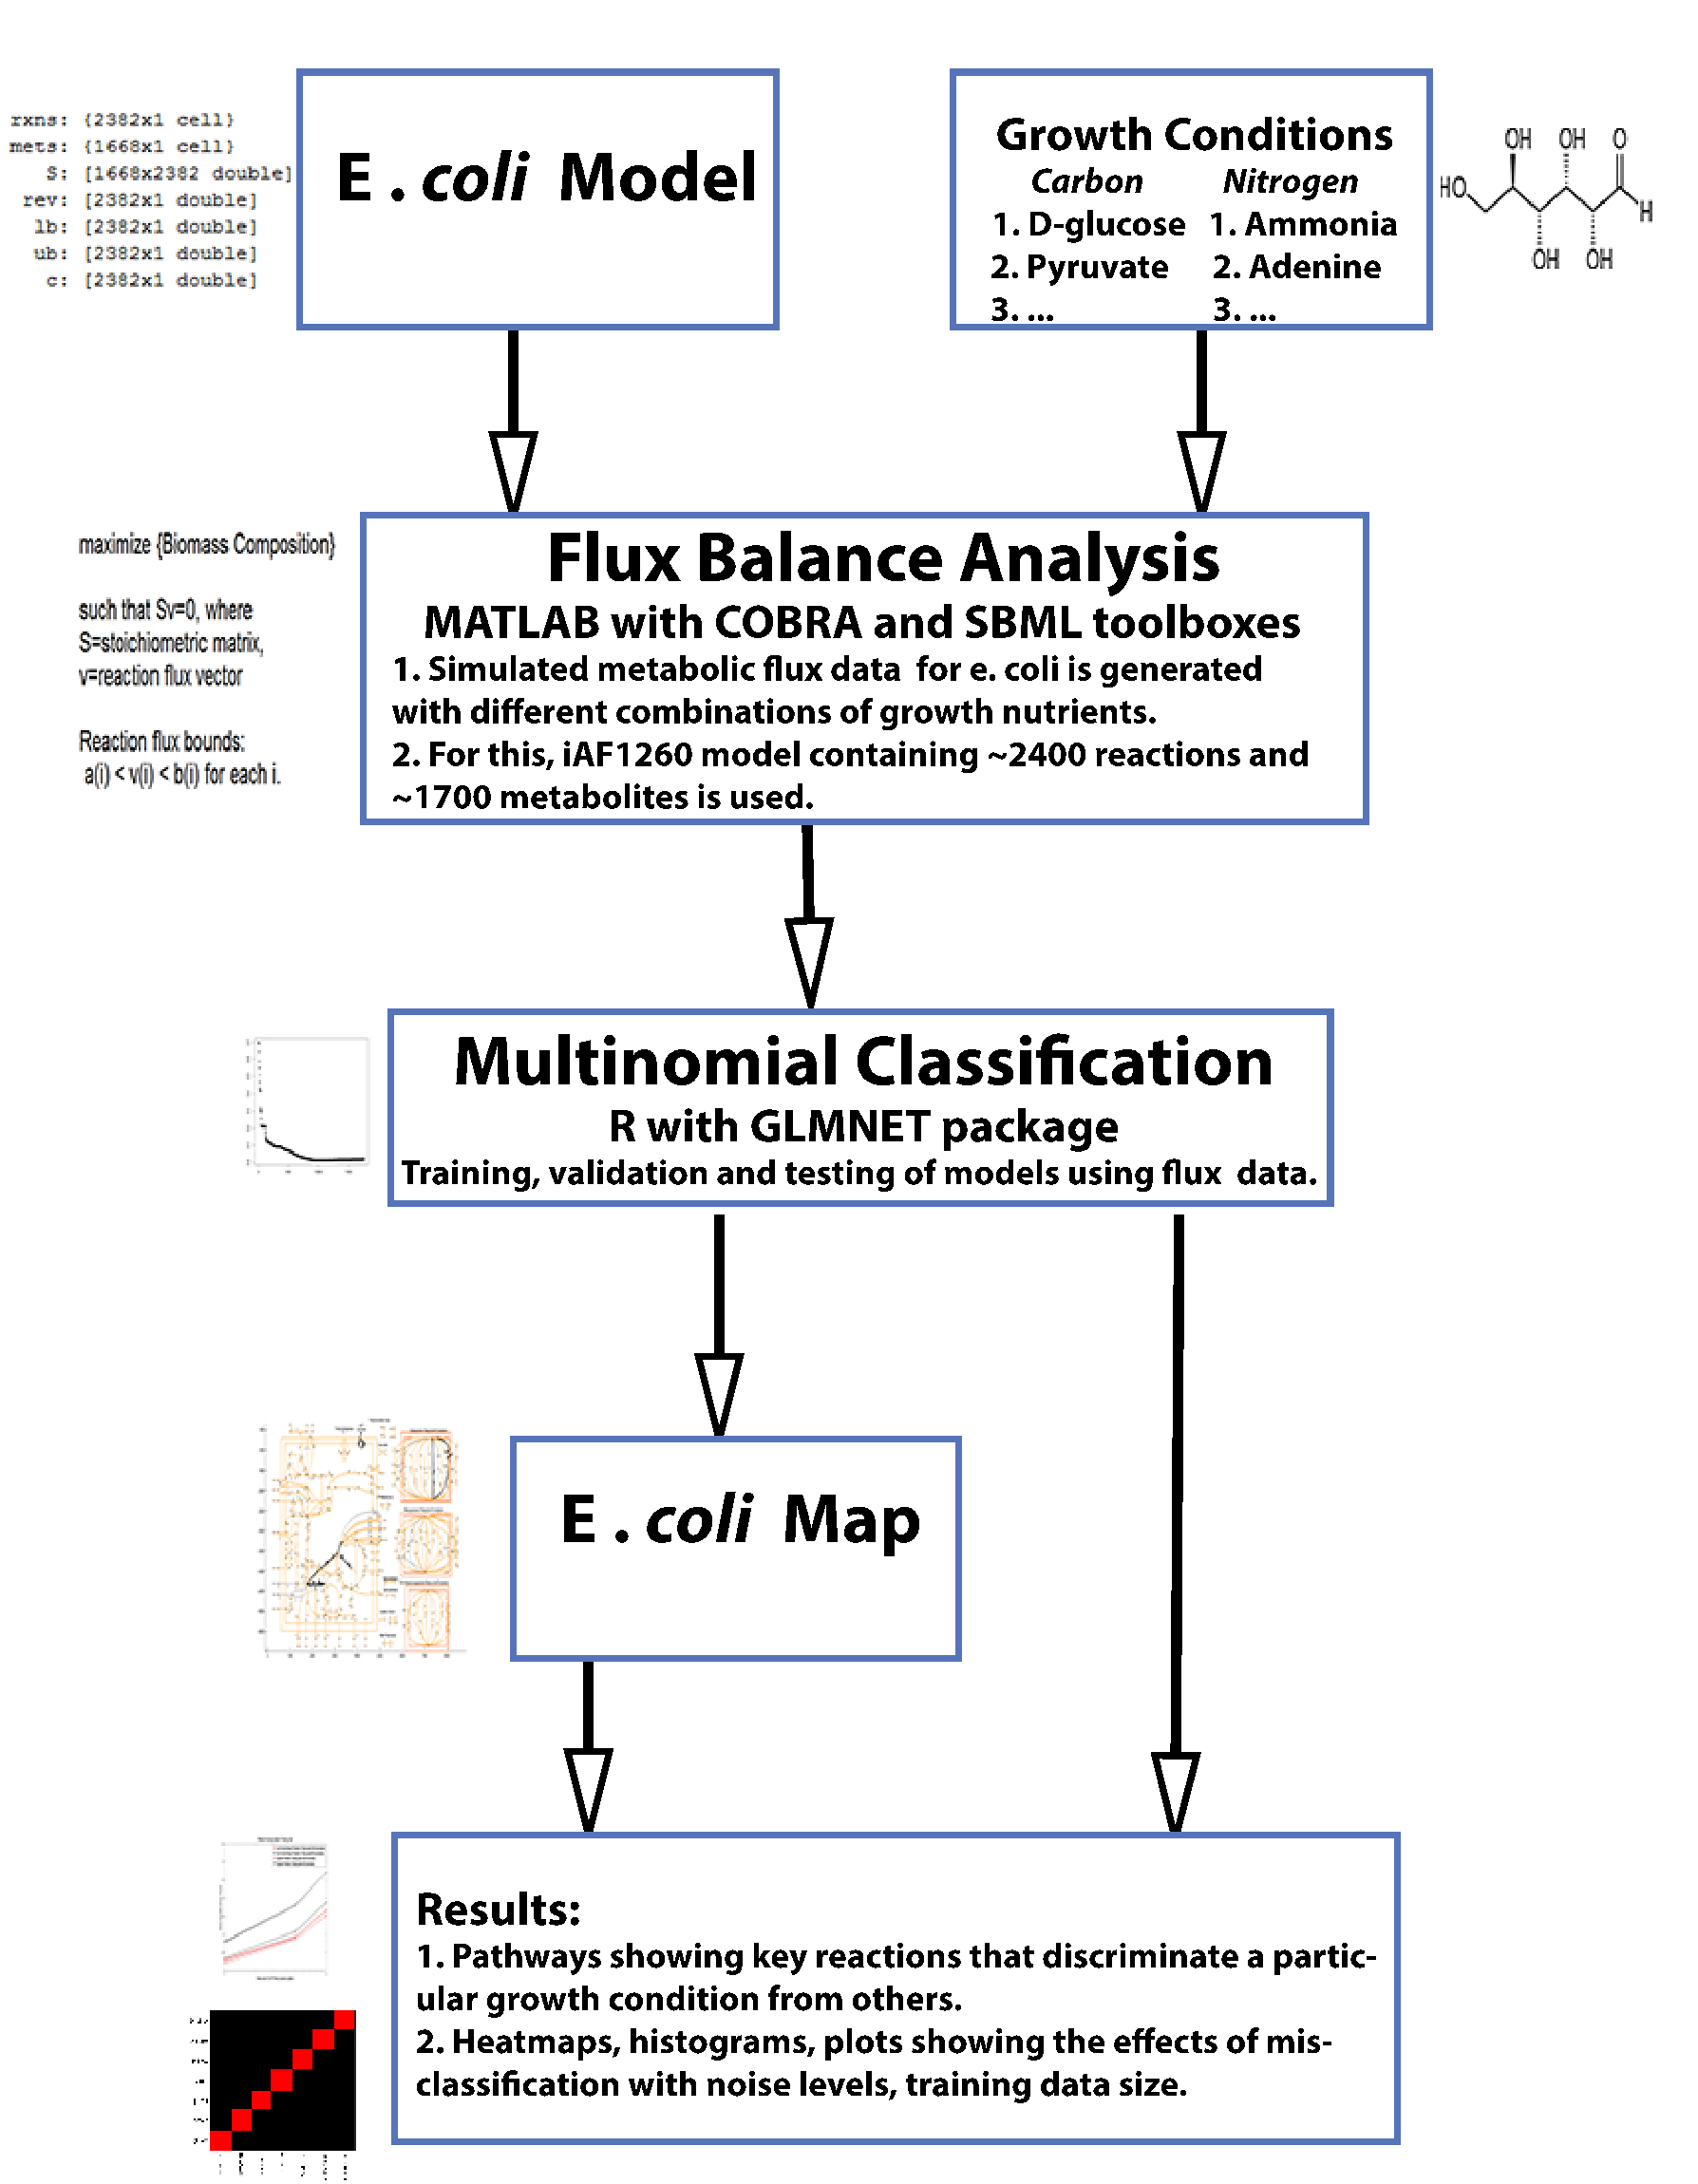
\includegraphics[width=4in]{Figures/flowchart_new.pdf}}
\caption{\label{fig:flowchart}\title{Flowchart describing methodology used in this study.} We obtained E. coli model and map from BiGG database. The key steps involved are Flux Balance Analysis and multinomial classification routines.}
\end{figure}

\clearpage
\begin{figure}[!ht]
\centerline{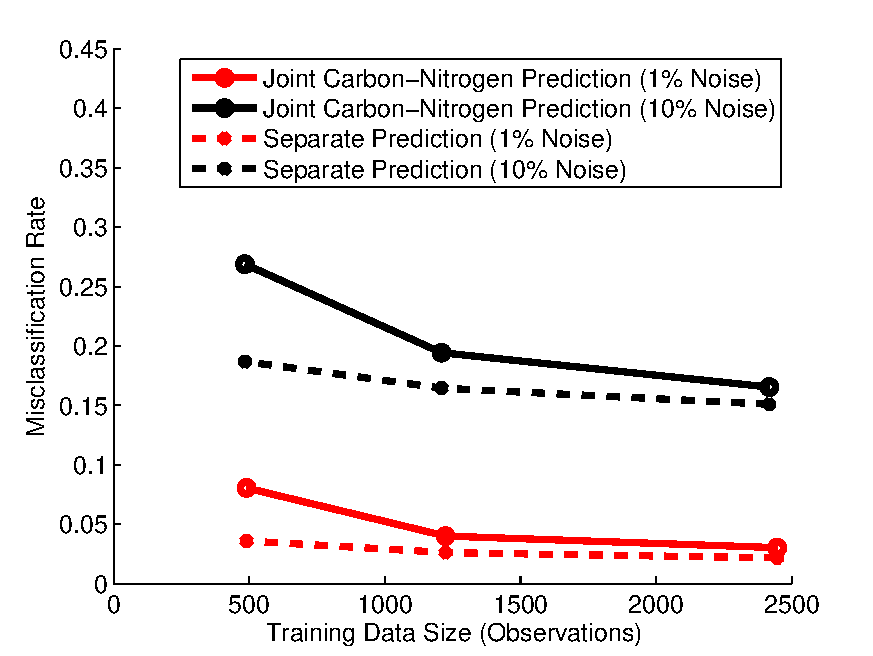
\includegraphics[width=6in]{Figures/VaryingData.pdf}}
\caption{\label{fig:misclassification_1}\title{Misclassification rate for different replicate sizes.} This plot shows that as training data size increases, the misclassification rate increases. This is tested for 2 different noise levels (1\% and 10\%).}
\end{figure}

\clearpage
\begin{figure}[!ht]
\centerline{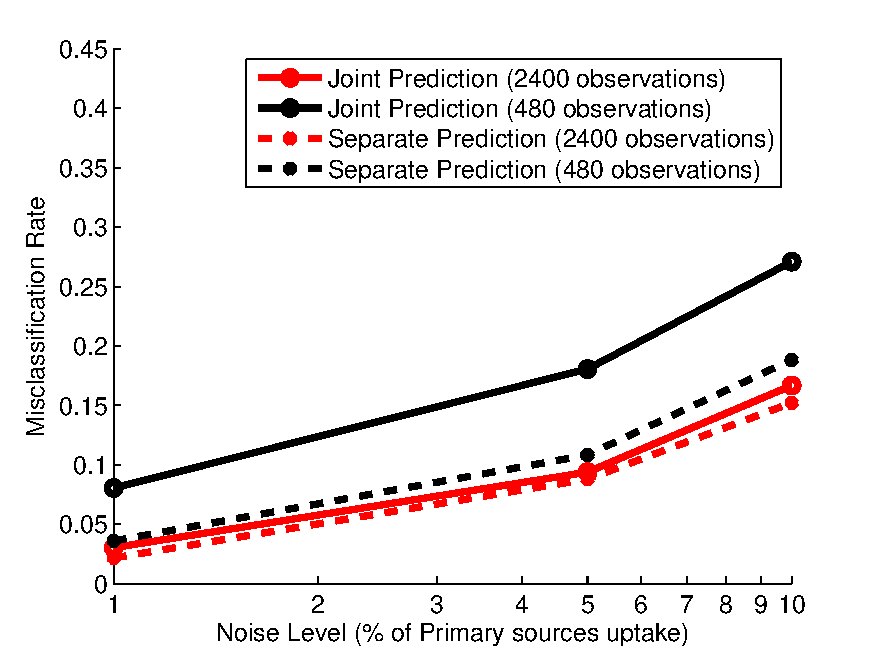
\includegraphics[width=6in]{Figures/VaryingNoise.pdf}}
\caption{\label{fig:misclassification_2}\title{Misclassification rate at different noise levels.} This plot shows that misclassification rate increases as noise increases in FBA models. This is tested for 2 different replicate sizes (480 and 2400 observations).}
\end{figure}

\clearpage
\begin{figure}[p]
\centerline{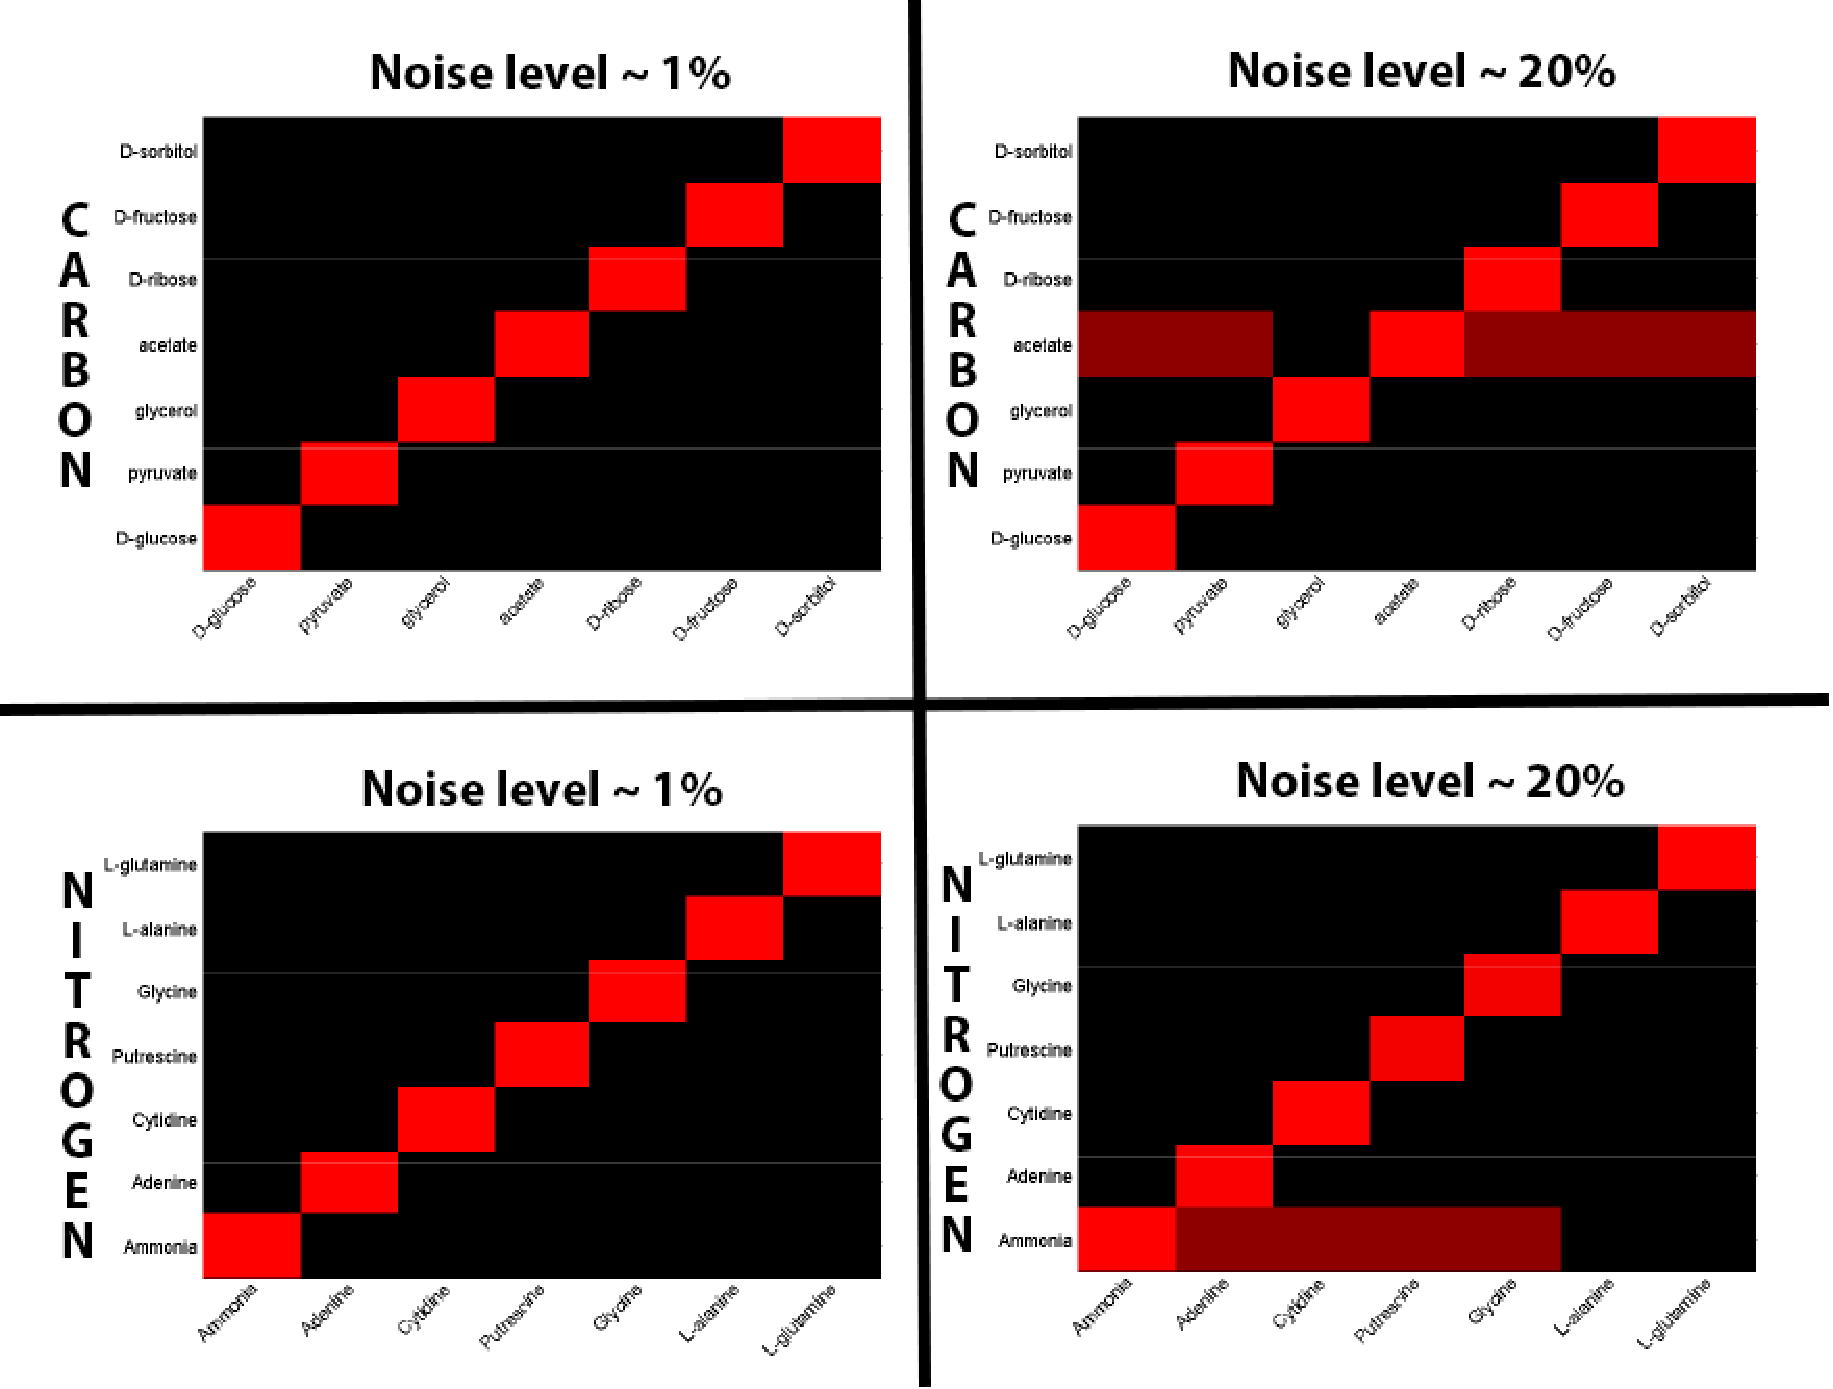
\includegraphics[width=6in]{Figures/heatmap.pdf}}
\caption{\label{fig:heat_map}\title{Heat maps with actual sources as columns and predicted ones in rows.}  At 20\% noise, most C sources are predicted to be acetate and most N sources are predicted to be ammonia.}
\end{figure}

\clearpage
\begin{figure}[p]
\centerline{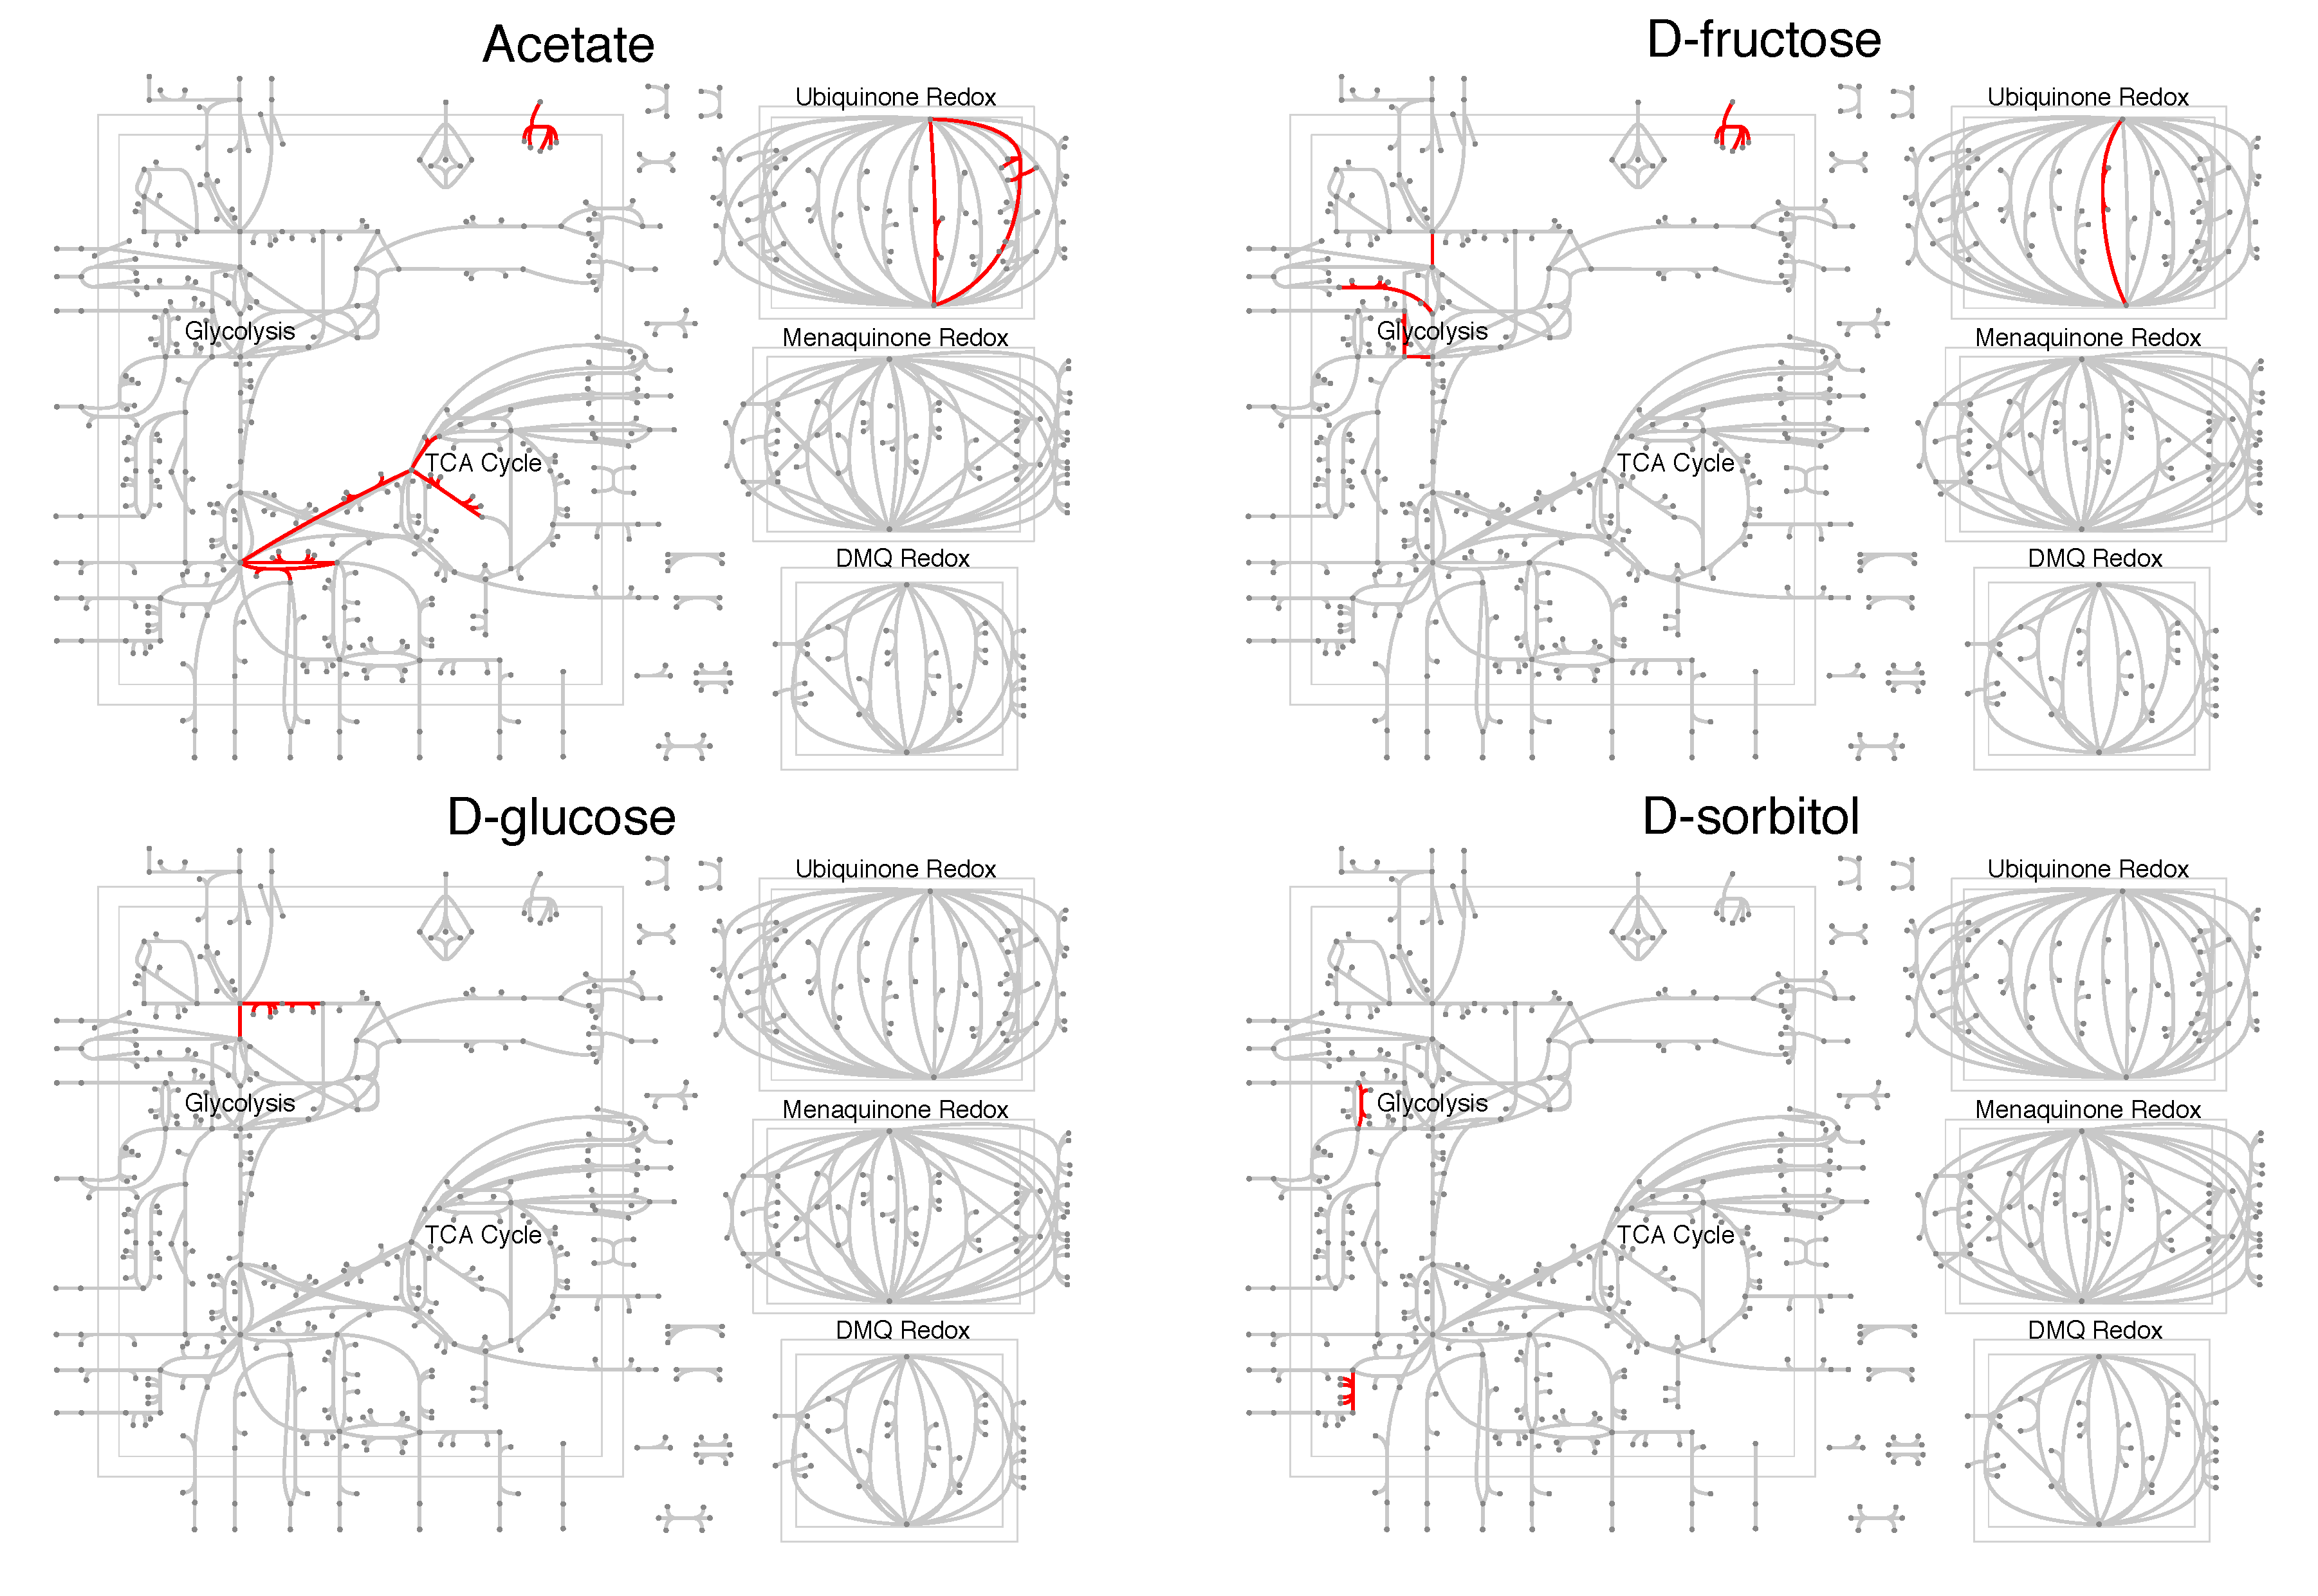
\includegraphics[width=7in]{Figures/carbon/carbon_grid.pdf}}
\caption{\label{fig:carbon_network}\title{Discriminatory carbon sources} The key-reactions identified by GLMNET package were mapped onto E. coli central metabolism to visually show the differences between different growth conditions. Out of 7 carbon sources, here we show 4 carbon sources and the key-reactions.}
\end{figure}

\clearpage
\begin{figure}[p]
\centerline{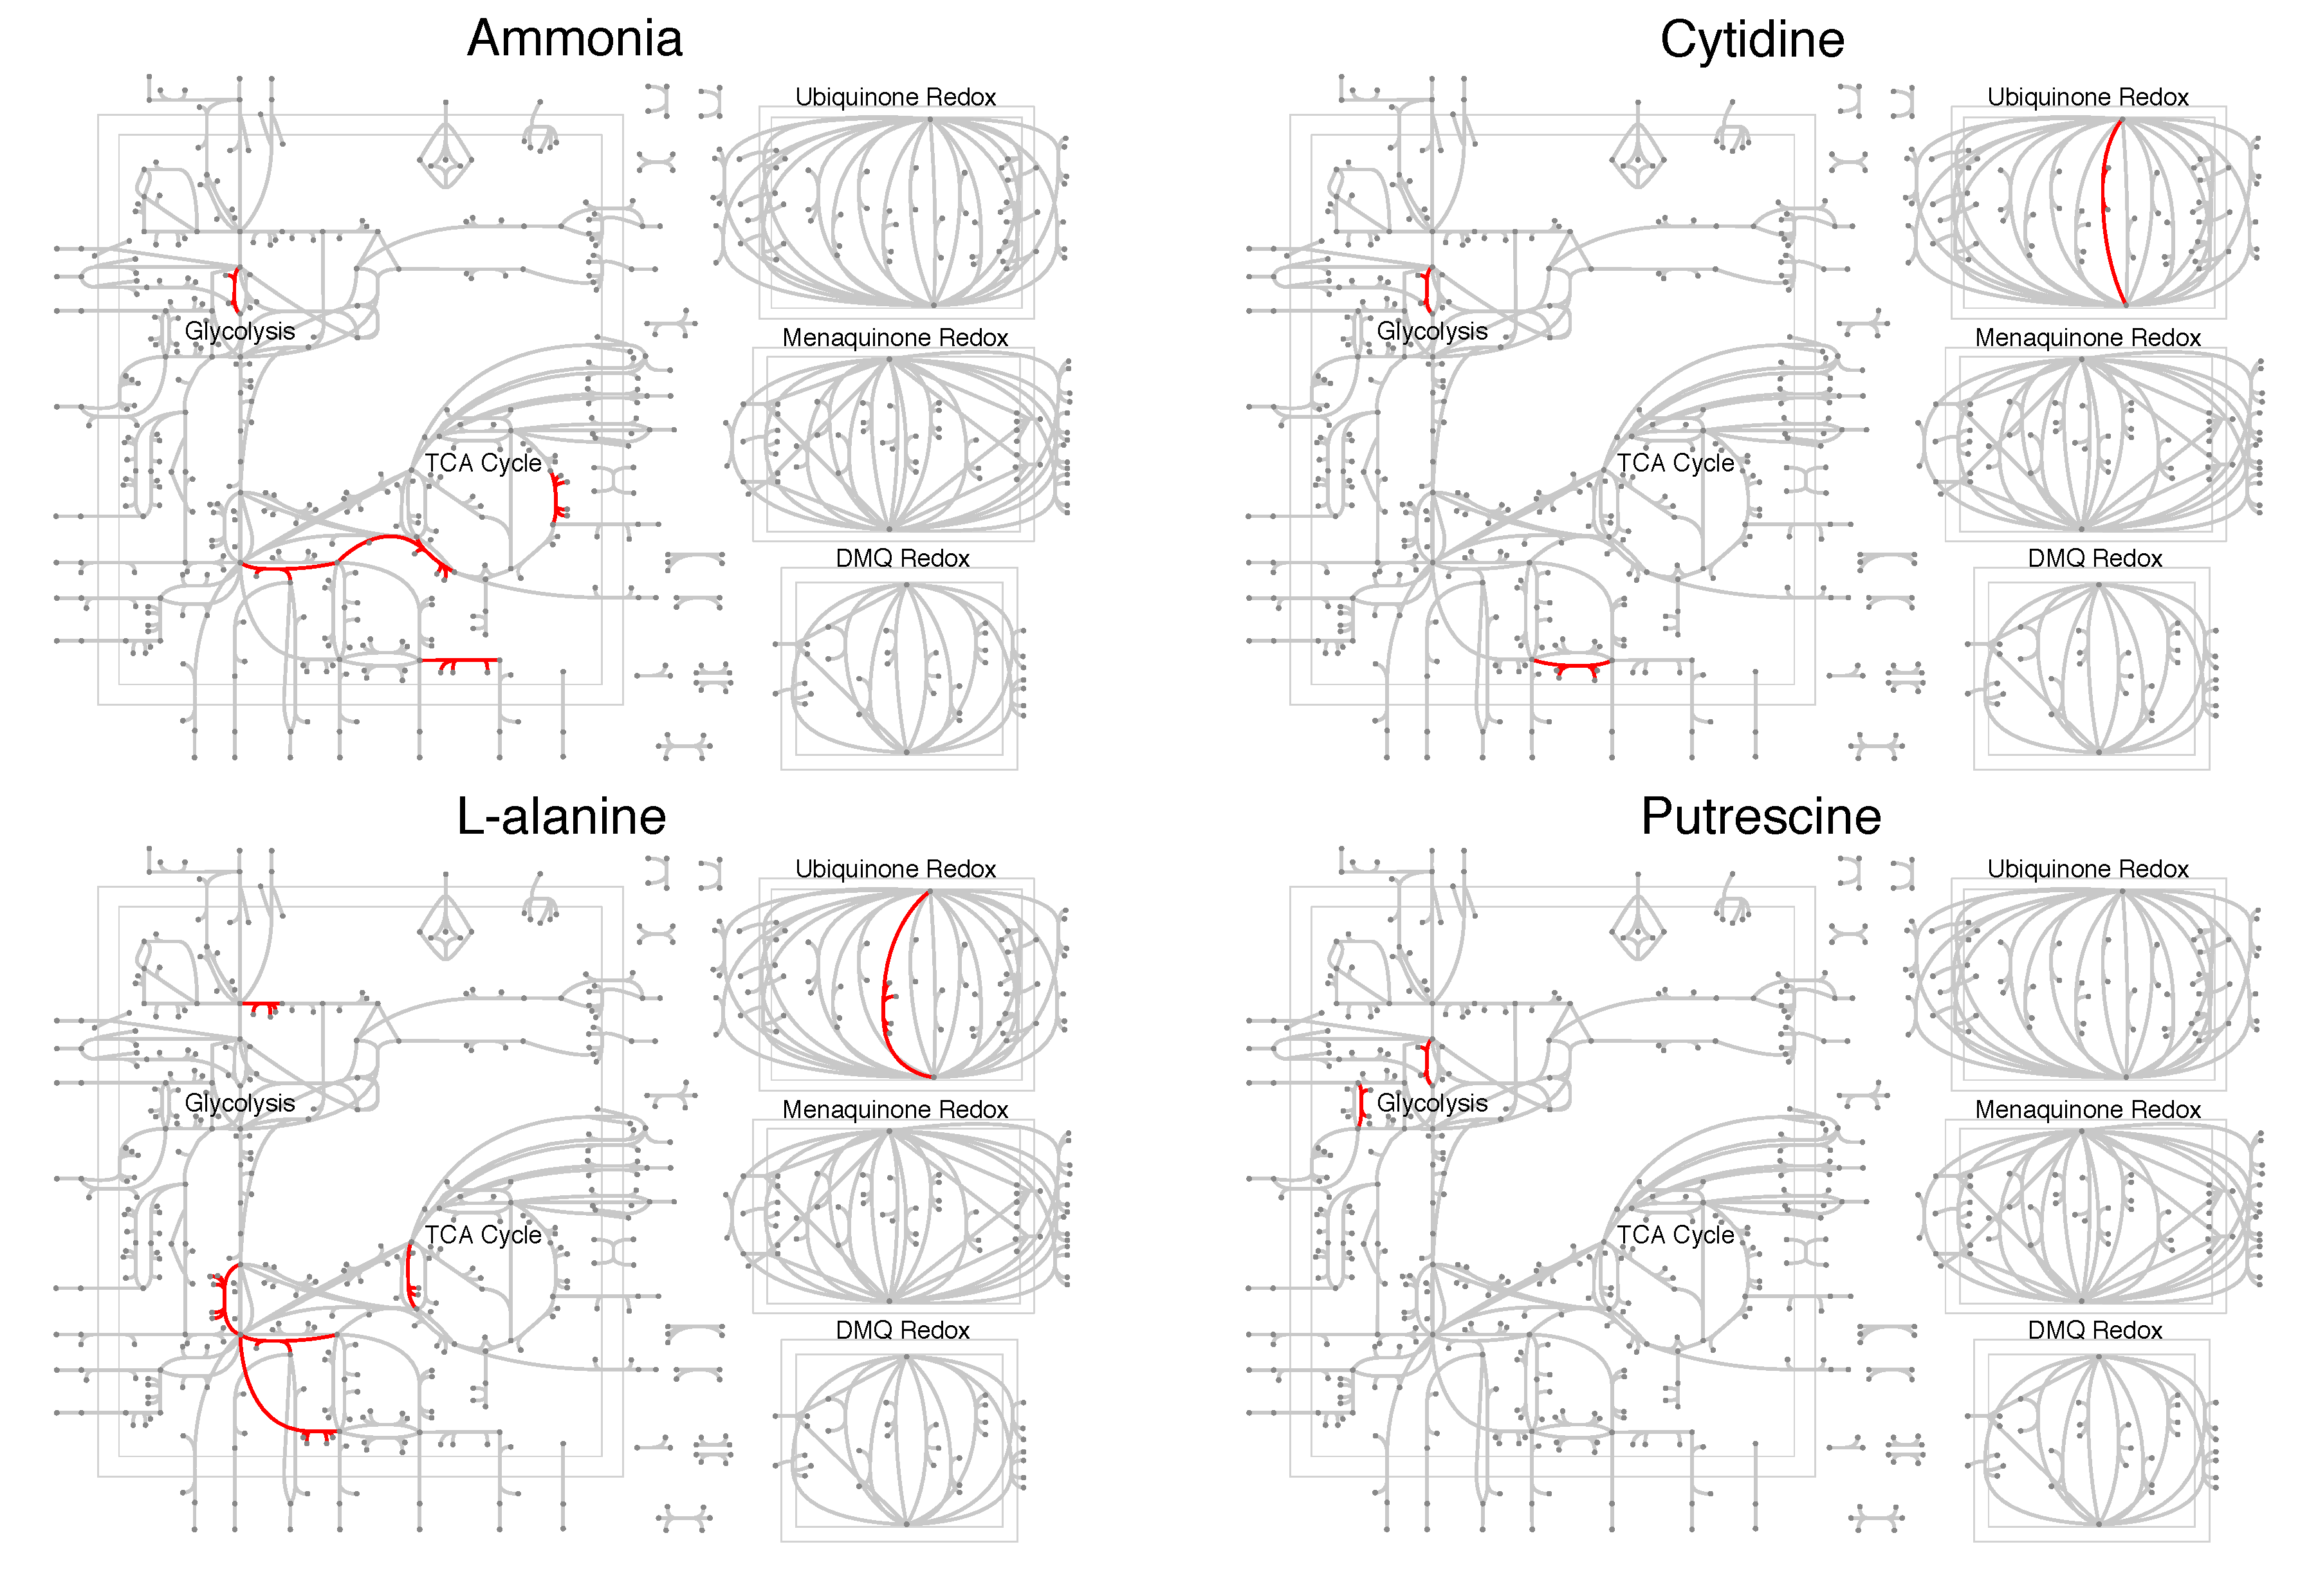
\includegraphics[width=7in]{Figures/nitrogen/nitrogen_grid.pdf}}
\caption{\label{fig:nitrogen_network}\title{Discriminatory nitrogen sources} The key-reactions identified by GLMNET package were mapped onto E. coli central metabolism to visually show the differences between different growth conditions. Here, the growth medium used are generally used for K-12 MG1655 strain.}
\end{figure}

\end{document}
